\chapter{Módulo: Personal}
\label{mod:03-personal}

\section{Propósito}
\label{sec:personal-proposito}

Gestiona al personal administrativo/operativo de la óptica (recepción, cajeros, vendedores, etc.) que necesita acceso al sistema pero no es un profesional de salud --- es la contraparte de RR.HH.\ de \code{Professional}. Alimenta al módulo de Egresos (\code{SalarioEmpleado}) para el registro de nóminas.

\section{Entidades principales}
\label{sec:personal-entidades}

Ver Capítulo~\ref{sec:modelo-datos}, Grupo A.

\begin{longtable}{p{3.2cm}p{10.1cm}}
\caption{Entidades principales del módulo de Personal.}\label{tab:personal-entidades}\\
\toprule
\textbf{Entidad} & \textbf{Rol} \\
\midrule
\endfirsthead
\toprule
\textbf{Entidad} & \textbf{Rol} \\
\midrule
\endhead
\bottomrule
\endfoot
\code{Empleado} & Marca que un \code{User} es empleado. \code{CargoId} FK, \code{FechaIngreso}/\code{FechaEgreso}, \code{SalarioBase} nullable. \\
\code{CargoEmpleado} & Catálogo de cargos/puestos (ej.\ Recepcionista, Cajero). \\
\end{longtable}

\section{Reglas de negocio clave}
\label{sec:personal-reglas}

\begin{itemize}
  \item \textbf{Estructura idéntica a \code{Professional}:} \code{Empleado} siempre requiere \code{User} (1:1), se crea con \code{Is}\allowbreak \code{Email}\allowbreak \code{Verified=true} y \code{Must}\allowbreak \code{Change}\allowbreak \code{Password=true} en la misma transacción (\code{Person}+\code{User}+\code{Empleado}+asignación de rol) --- mismo patrón que el alta de profesional (Capítulo~\ref{mod:02-pacientes-y-profesionales}).
  \item \textbf{\code{CargoEmpleado} es un catálogo simple sin controller propio} --- se gestiona como sub-recurso de \code{Empleados}\allowbreak \code{Controller} (\code{/}\allowbreak \code{api/}\allowbreak \code{empleados/}\allowbreak \code{cargos}), no tiene su ruta base independiente.
  \item \textbf{La sucursal del empleado se asigna en este mismo formulario} (\code{EmpleadosView}), igual que para profesionales --- no desde \code{UsuariosView}.
  \item \textbf{\code{SalarioBase} es nullable y opcional} --- no todo empleado tiene un salario fijo cargado aquí; cuando existe, es la base que consume el módulo de Egresos para generar \code{SalarioEmpleado} (un \code{Egreso} de tipo salario). Ver Capítulo~\ref{mod:11-caja-y-egresos}.
  \item \textbf{\code{FechaEgreso} nullable} --- permite registrar la baja de un empleado sin necesariamente desactivar el \code{User} en el mismo momento (son dos campos independientes: la fecha de egreso es dato de RR.HH., \code{IsActive} del \code{User} es control de acceso).
  \item \textbf{Borrado lógico} vía desactivación del \code{User} asociado, igual que el resto de las cuentas de staff.
\end{itemize}

\section{Endpoints}
\label{sec:personal-endpoints}

Detalle completo en el Apéndice de Referencia de API, \S 3 (\code{Empleados}\allowbreak \code{Controller}, que usa su propio \code{ToResponse} en vez de \code{BaseController} --- única excepción en los 37 controllers).

\begin{longtable}{p{3.6cm}p{4.6cm}p{5.1cm}}
\caption{Endpoints principales del módulo de Personal.}\label{tab:personal-endpoints}\\
\toprule
\textbf{Método} & \textbf{Ruta} & \textbf{Descripción} \\
\midrule
\endfirsthead
\toprule
\textbf{Método} & \textbf{Ruta} & \textbf{Descripción} \\
\midrule
\endhead
\bottomrule
\endfoot
GET & \code{/}\allowbreak \code{api/}\allowbreak \code{empleados?soloActivos} & Listado \\
POST/PUT/DELETE & \code{/api/empleados} & Alta (transacción multi-entidad), edición, desactivación \\
GET/POST/PUT & \code{/}\allowbreak \code{api/}\allowbreak \code{empleados/}\allowbreak \code{cargos} & Catálogo de cargos, anidado bajo este mismo controller \\
\end{longtable}

\section{Flujo típico}
\label{sec:personal-flujo}

Idéntico en estructura al alta de profesional (ver el diagrama de secuencia del Capítulo~\ref{mod:02-pacientes-y-profesionales}), reemplazando \code{Professional}/\code{LicenseNumber}/\code{Profesional}\allowbreak \code{Especialidad} por \code{Empleado}/\code{CargoId}/\code{FechaIngreso}. No se repite el diagrama aquí para no duplicar contenido --- la única diferencia estructural es que no hay equivalente a ``especialidades'' (many-to-many), la relación con \code{CargoEmpleado} es N:1 simple.

\section{Vistas de frontend}
\label{sec:personal-vistas}

\begin{itemize}
  \item \code{EmpleadosView.vue}
  \item \code{CargosEmpleadoView.}\allowbreak \code{vue}
\end{itemize}

\section{Interfaz}
\label{sec:personal-interfaz}

\begin{figure}[htbp]
\centering
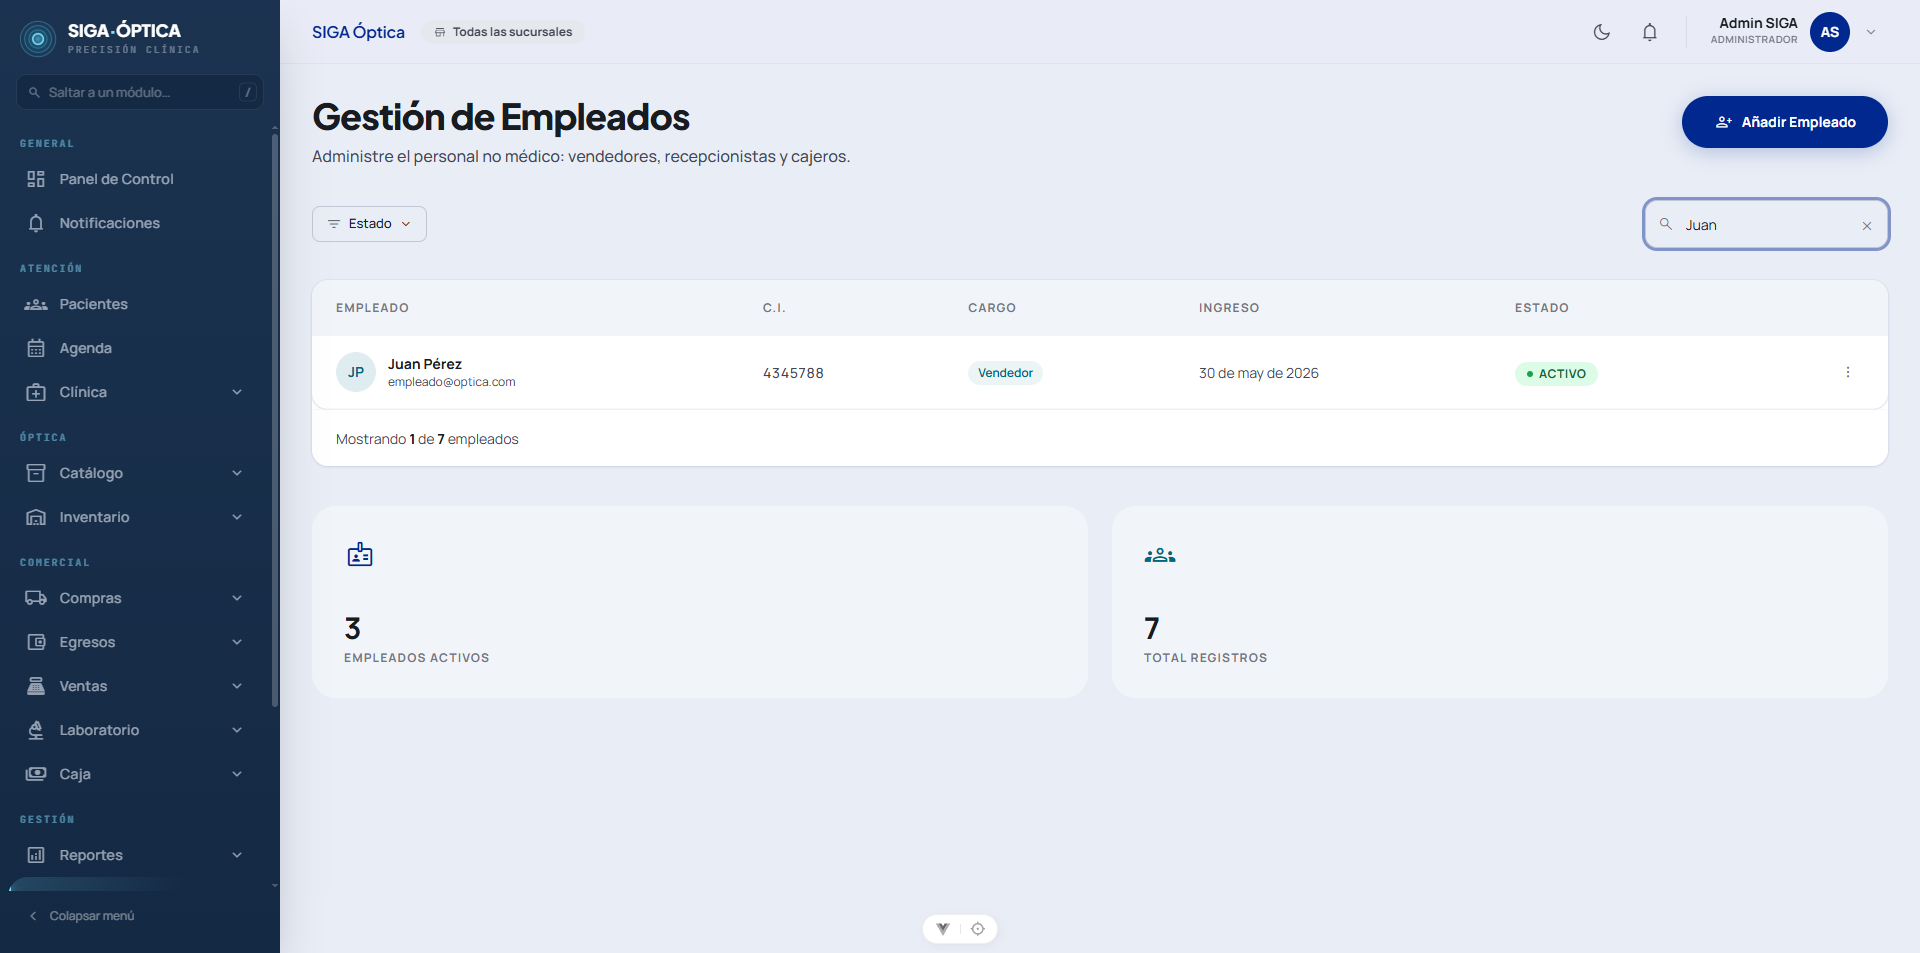
\includegraphics[width=0.95\textwidth]{imagenes/mod03-empleados.png}
\caption{Gestión de empleados administrativos, con su cargo, fecha de ingreso y estado.}
\label{fig:mod03-empleados}
\end{figure}

\section{Estado}
\label{sec:personal-estado}

\Implementado. Sin limitaciones conocidas específicas de este módulo más allá de las ya generales de gestión de cuentas (Capítulo~\ref{mod:01-identidad-y-acceso}, \S\ref{sec:identidad-estado}).
